\documentclass[11pt,notes=hide,aspectratio=169,mathserif]{beamer}

% PACKAGES
\usepackage{graphics}  % Support for images/figures
\usepackage{graphicx}  % Includes the \resizebox command
\usepackage{tikz}      % For flowcharts
\usetikzlibrary{arrows.meta, positioning} % Libraries for TikZ


\usepackage{url}	   % Includes \urldef and \url commands
\usepackage{natbib}
\usepackage{bibentry}  % Includes the \nobibliography command
\usepackage{verbatim}  %Supports comments
\usepackage{booktabs} %Supports \toprule, \bottomrule, etc in tables
\usepackage{etoolbox}  %Supports toggle commands
\usepackage{datetime}
\usepackage{bm}	%Supports bold math \bm
%the LaTeX standard:
\usepackage{cmbright}
\setbeamerfont{frametitle}{family=\fontfamily{cmbr}\selectfont,size=\Large}
\fontencoding{OT1}\fontfamily{cmbr}\selectfont

% PACKAGES (that should already be included by your LyX document settings)
\usepackage{amsfonts}  % Lots of stuff, including \mathbb 
\usepackage{amsmath}   % Standard math package
\usepackage{amsthm}    % Includes the comment functions
\usepackage{subcaption}

% CUSTOM DEFINITIONS
\def\newblock{} %Get beamer to cooperate with BibTeX
\linespread{1.2}

% IDENTIFYING INFORMATION
\title[class]{ECON 326: Economics of Developing Countries \\ TA Session 9}
\author[vaidehi's class ]{Vaidehi Parameswaran (Northwestern Econ)}
\date{\monthname[\the\month] \the\year}

% THEMATIC OPTIONS
%\setbeamercovered{transparent}
\usetheme{metropolis}
\definecolor{mycolor}{RGB}{0,153,153} % define cyan colour
\setbeamercolor{frametitle}{bg=mycolor, fg=white} % Frame title color
\setbeamercolor{title separator}{fg=mycolor} 
\setbeamercolor{progress bar}{fg=mycolor} 
\beamertemplatenavigationsymbolsempty
%\setbeamertemplate{footline}[frame number]{}
\setbeamertemplate{itemize item}{\small\raisebox{1pt}{\textcolor{mycolor}{$\blacktriangleright$}}}
\setbeamertemplate{itemize subitem}{\footnotesize\raisebox{1pt}{\textcolor{mycolor}{$\triangleright$}}}
\setbeamertemplate{itemize subsubitem}{\tiny\raisebox{1pt}{\textcolor{mycolor}{$\triangleright$}}}

% BACKUP SLIDE NUMBERING
\usepackage{appendixnumberbeamer}

\begin{document}

%---------------------------------------------------------------------
\begin{frame}[plain]
\titlepage
\end{frame}
%---------------------------------------------------------------------


%---------------------------------------------------------------------
\begin{frame}{Today's Agenda}

\begin{itemize}
\item \href{https://www.lse.ac.uk/economics/Assets/Documents/personal-pages/robin-burgess/the-brazilian-amazons-double-reversal-of-fortune-manuscript.pdf}{\textcolor{blue}{Burgess et al. (2019)}}
\item The Curse of Natural Resources
\item Practice final
\end{itemize}
\end{frame}
%---------------------------------------------------------------------


\section*{\href{https://www.lse.ac.uk/economics/Assets/Documents/personal-pages/robin-burgess/the-brazilian-amazons-double-reversal-of-fortune-manuscript.pdf}{\textcolor{blue}{Burgess et al. (2019)}} \\[5mm] 
\textnormal{\small{The Brazilian Amazon’s Double Reversal of Fortune}}}

%---------------------------------------------------------------------
\begin{frame}{Motivation}
\begin{itemize}
\item Environmental damage entails an externality - a market failure 
\item Requires government involvement to regulate or tax activity to correct this externality
\item State capacity to effectively regulate is weak in many developing countries
\item Political economy can be important 
\end{itemize}
\end{frame}
%---------------------------------------------------------------------

%---------------------------------------------------------------------
\begin{frame}{This Paper}
\begin{itemize}
\item Explore how national policies can exert regulatory control over conservation 
\item Exploit what happens at international borders 
\item One of the most important global ecosystems: the Amazon rainforest
\begin{itemize}
    \item The rate of deforestation will affect global warming
    \item The Amazon is a global public good
\end{itemize}
\end{itemize}
\end{frame}
%---------------------------------------------------------------------

%---------------------------------------------------------------------
\begin{frame}{Strategy}
\begin{itemize}
\item Satellite data on deforestation - even across borers, from 2000 - 2018 
\begin{itemize}
\item High resolution - can zoom in for precise effects 
\end{itemize}
\item In 2006, Brazil introduced deforestation policies
\item Spatial RDD design - popular strategy using borders for policy effects
\end{itemize}
\end{frame}
%---------------------------------------------------------------------

%---------------------------------------------------------------------
\begin{frame}{Satellite Data}
\begin{figure}
\centering
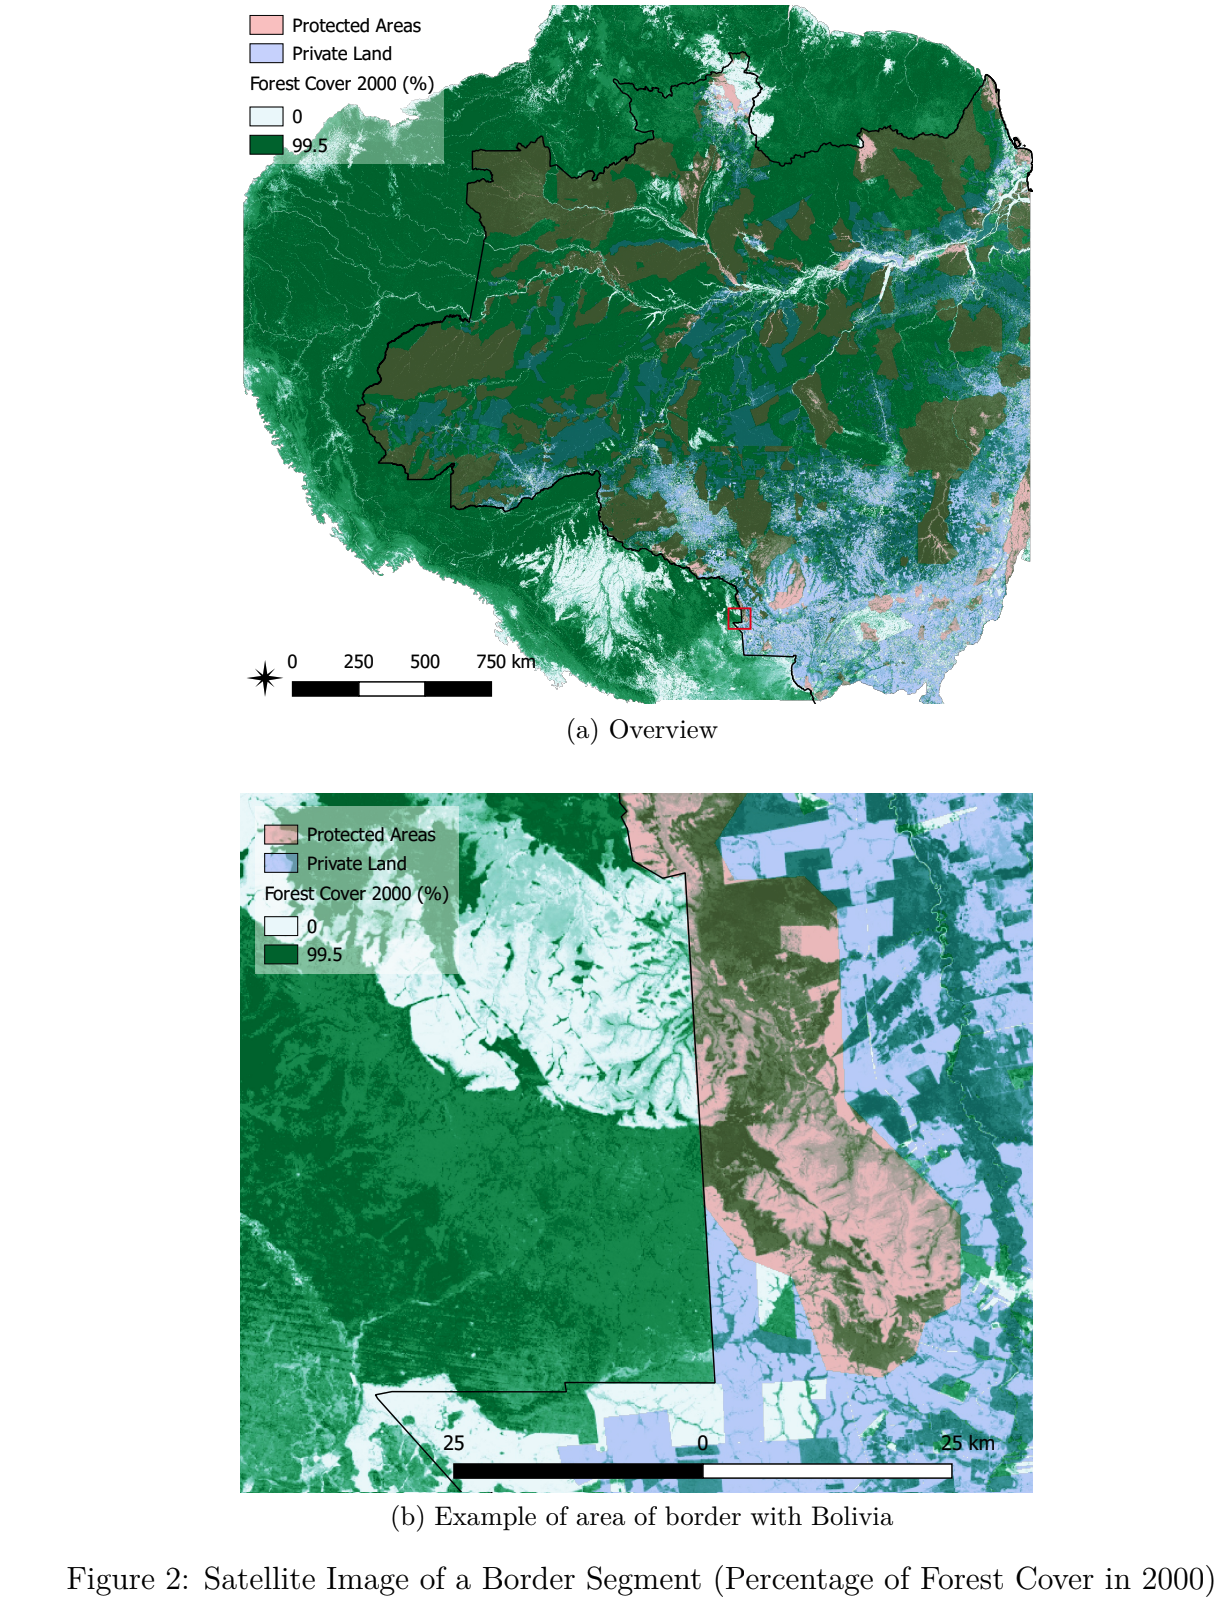
\includegraphics[width=0.4\textwidth]{../TA9/inputs/fig2.2.png}
\end{figure}
\end{frame}
%---------------------------------------------------------------------

%---------------------------------------------------------------------
\begin{frame}{Fact 1}
\begin{figure}
\centering
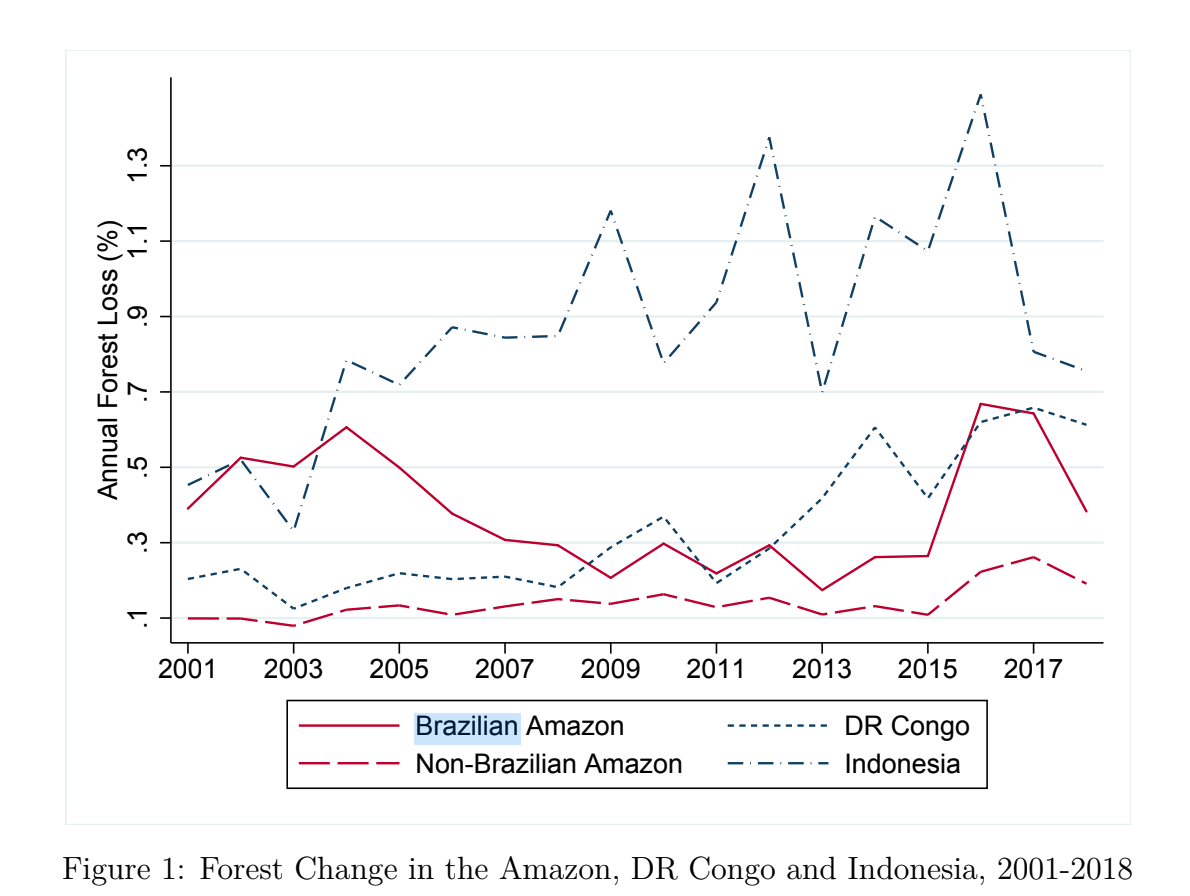
\includegraphics[width=0.6\textwidth]{../TA9/inputs/fig2.1.png}
\end{figure}
\begin{itemize}
\item Until 2005, deforestation level and rate significantly higher on the Brazilian side 
\end{itemize}
\end{frame}
%---------------------------------------------------------------------

%---------------------------------------------------------------------
\begin{frame}{Fact 1}
\begin{figure}
\centering
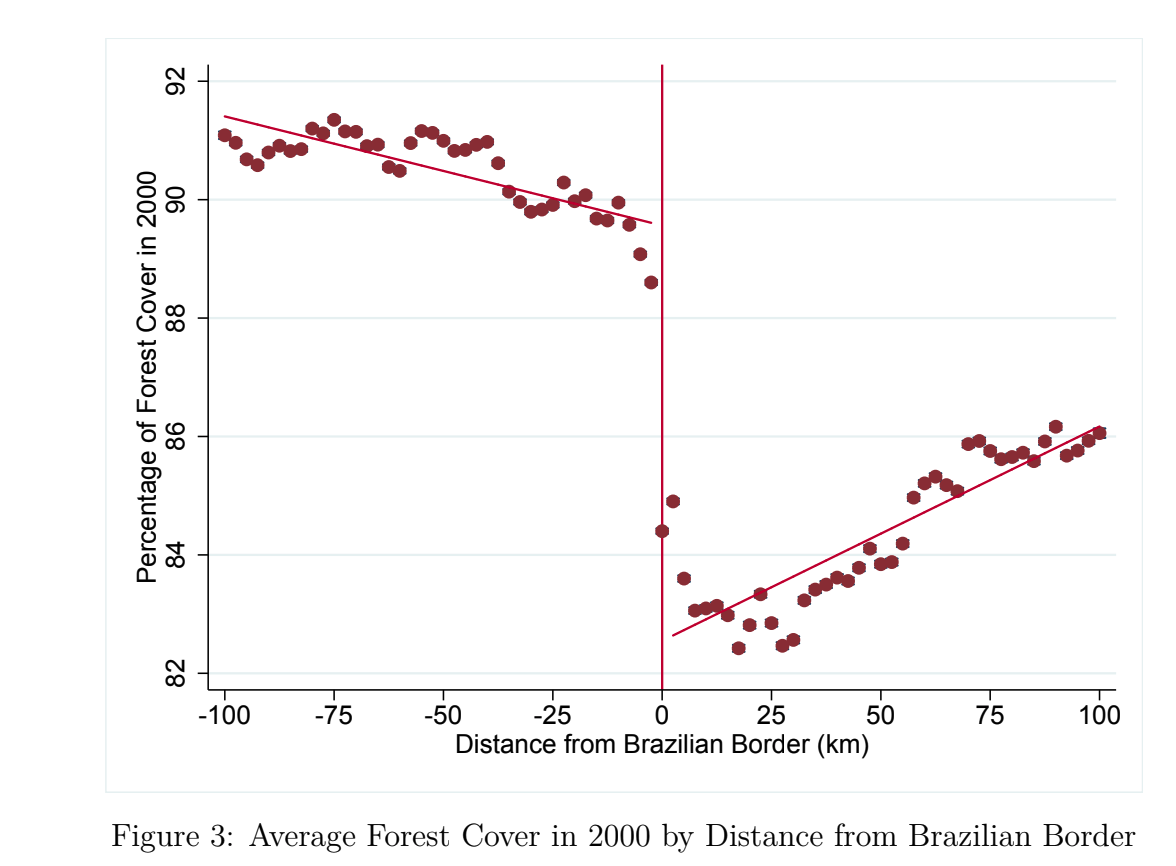
\includegraphics[width=0.56\textwidth]{../TA9/inputs/fig2.3.png}
\end{figure}
\begin{itemize}
\item Deforestation is visually apparent: forest cover drops sharply exactly at the national border.
\end{itemize}
\end{frame}
%---------------------------------------------------------------------


%---------------------------------------------------------------------
\begin{frame}{Fact 2}
\begin{figure}
\centering
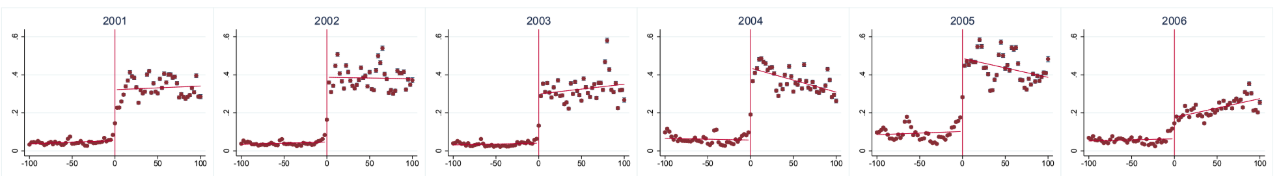
\includegraphics[width=1\textwidth]{../TA9/inputs/fig_2006.png}
\end{figure}
\begin{itemize}
\item Discontinuity in deforestation rates disappears in 2006 - the first reversal 
\end{itemize}
\end{frame}
%---------------------------------------------------------------------

%---------------------------------------------------------------------
\begin{frame}{What happened in 2006?}
\begin{itemize}
\item In 2003, in the Lula government, Marina Silva appointed as Minister of Environment
\item She was from the Amazon, and had a strong environmentalist stance
\item Law that allowed satellite-based deforestation detection system (DETER) to become a key tool
\item Sent in federal police and troops to arrest illegal loggers and confiscate their machinery
\end{itemize}
\end{frame}
%---------------------------------------------------------------------

%---------------------------------------------------------------------
\begin{frame}{Fact 3}
\begin{figure}
\centering
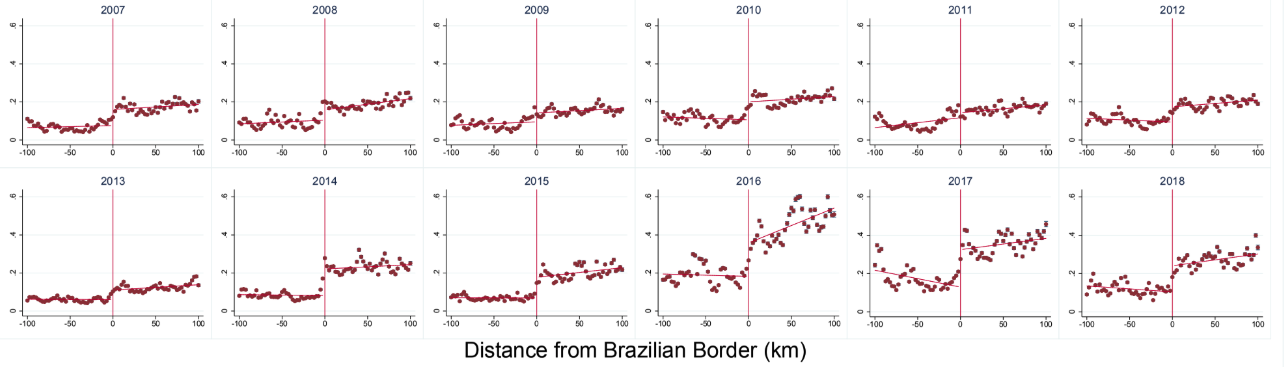
\includegraphics[width=1\textwidth]{../TA9/inputs/fig_post.png}
\end{figure}
\begin{itemize}
\item Positive effects relatively short-lived 
\item Deforestation resumes growing in 2014 - the second reversal
\end{itemize}
\end{frame}
%---------------------------------------------------------------------

%---------------------------------------------------------------------
\begin{frame}{What changed?}
\begin{itemize}
\item New government - gave amnesty to those engaged in illegal deforestation before 2008
\item 2014 was a politically turbulent year
\item Next president introduced laws that made it incentive-compatible for public land grabs
\end{itemize}
\end{frame}
%---------------------------------------------------------------------

%---------------------------------------------------------------------
\begin{frame}{The Double Reversal}
\begin{figure}
\centering
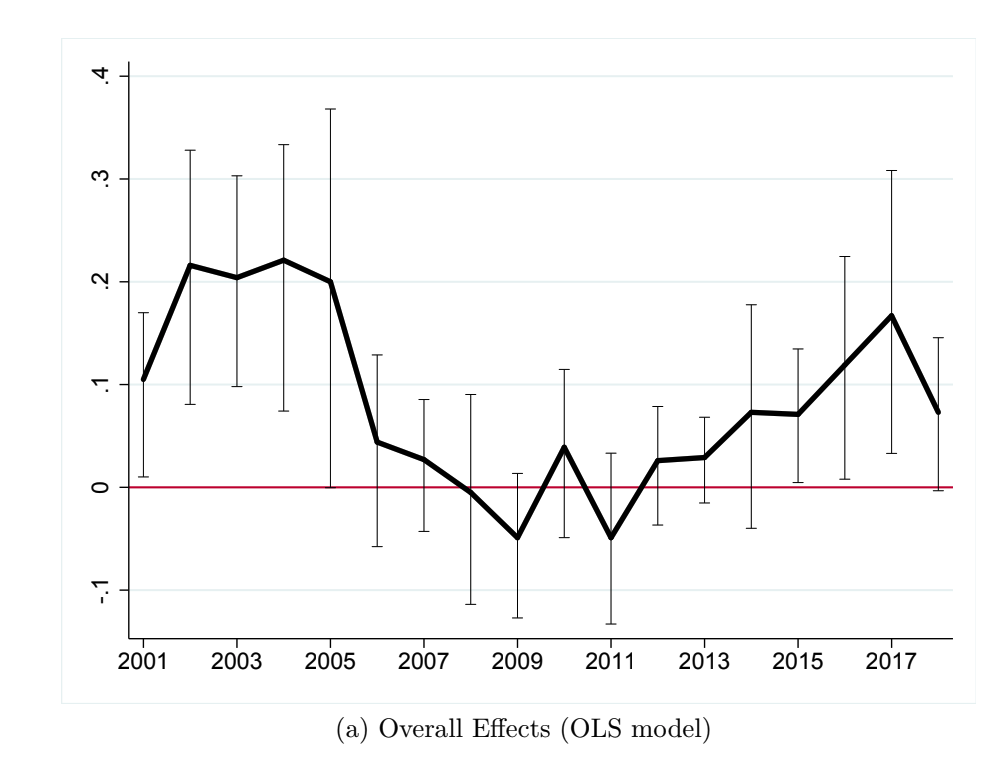
\includegraphics[width=0.6\textwidth]{../TA9/inputs/reversal.png}
\end{figure}
\end{frame}
%---------------------------------------------------------------------

%---------------------------------------------------------------------
\begin{frame}{Fact 4}
\begin{figure}
\centering
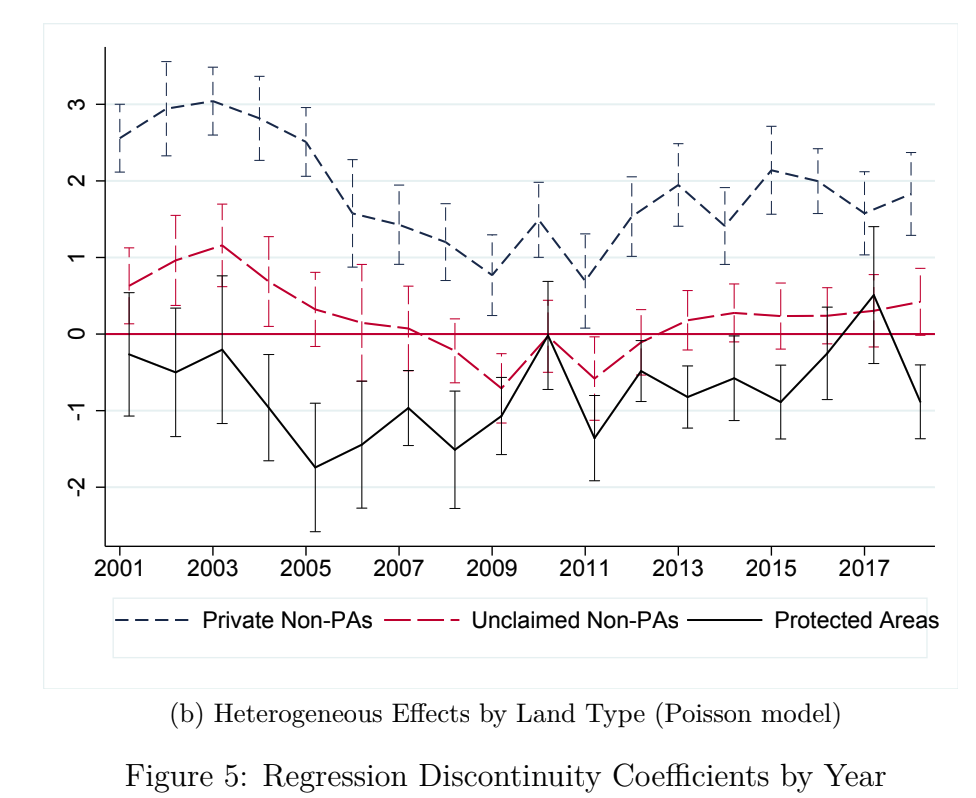
\includegraphics[width=0.5\textwidth]{../TA9/inputs/fig_land_use.png}
\end{figure}
\begin{itemize}
\item Land use restrictions matter 
\item Protected areas have always been less deforested
\end{itemize}
\end{frame}
%---------------------------------------------------------------------

%---------------------------------------------------------------------
\begin{frame}{Conclusion}
\begin{itemize}
\item Combined, these results demonstrate the reach of the Brazilian state to exploit or conserve its natural resources
\item Suggest that rapid deforestation in early 2000s was a consequence of a pro-exploitation policy environment 
\item Policy stance rapidly reversed in 2006-2013 with laws introduced 
\item But the position stalled and reversed in the post-2013 period with economic and political crisis collided with weakened forest conservation laws 
\item So state capacity does matter!
\end{itemize}
\end{frame}
%---------------------------------------------------------------------

\section*{The Curse of Natural Resources}

%---------------------------------------------------------------------
\begin{frame}{What is it?}

\begin{itemize}
\item The observation that countries rich in natural resources tend to perform badly
\item Also called the paradox of plenty or the resource curse
\item Sachs and Warner maybe the first to document this using econometrics in a paper in 1995
\end{itemize}
\end{frame}
%---------------------------------------------------------------------

%---------------------------------------------------------------------
\begin{frame}{Descriptive Evidence}
\begin{figure}
\centering
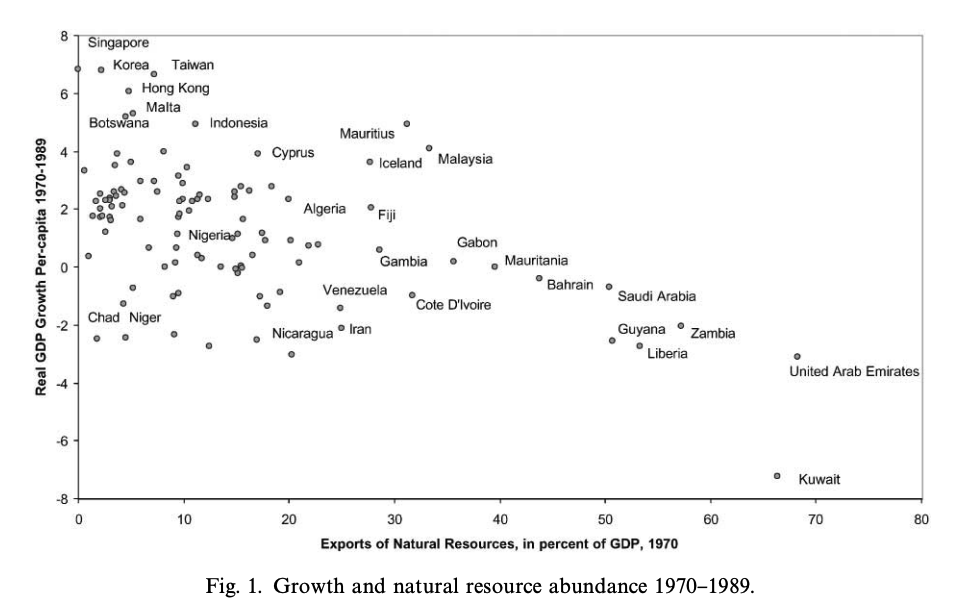
\includegraphics[width=0.6\textwidth]{../TA9/inputs/fig1.png}
\end{figure}
\begin{itemize}
\item No countries with extremely abundant natural resources in 1970 grew rapidly for the next 20 years
\end{itemize}
\end{frame}
%---------------------------------------------------------------------

%---------------------------------------------------------------------
\begin{frame}{Descriptive Evidence - Persistence}
\begin{figure}
\centering
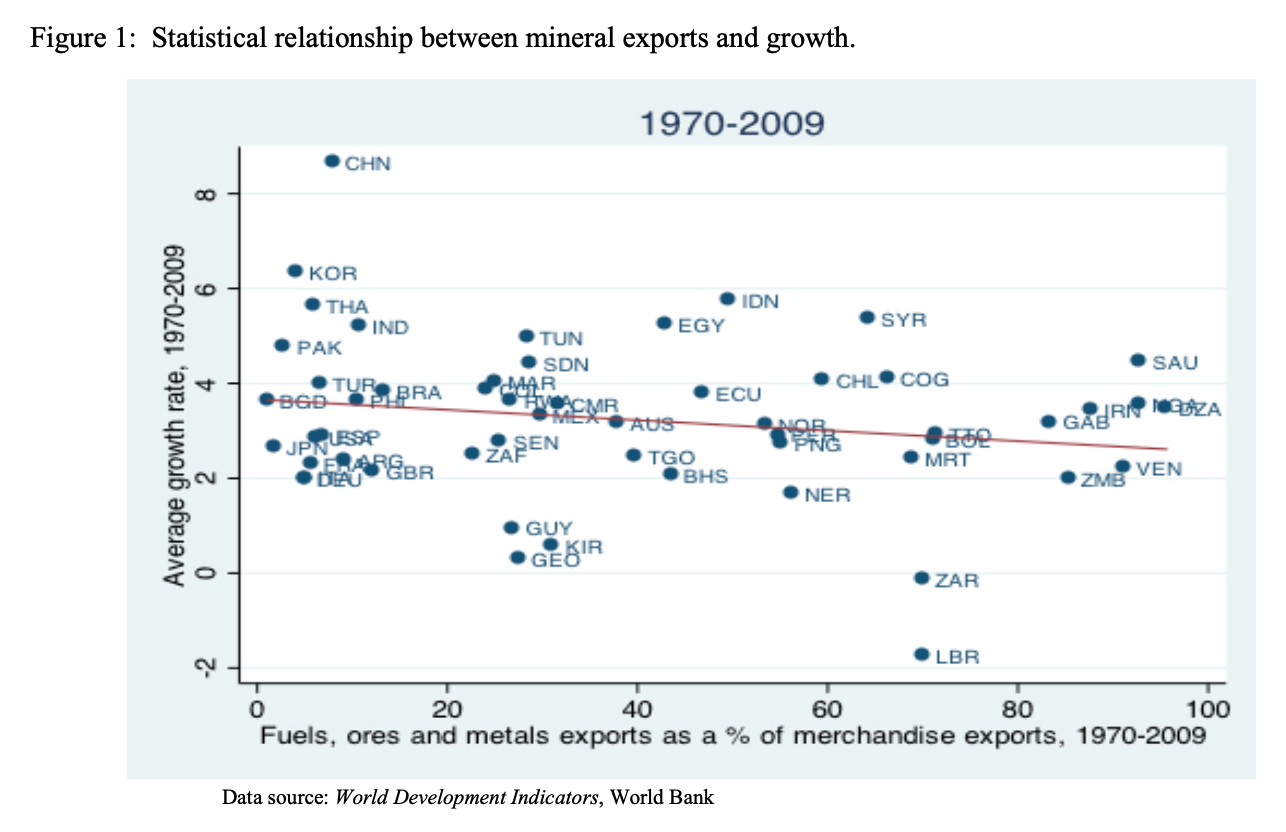
\includegraphics[width=0.55\textwidth]{../TA9/inputs/fig2.png}
\end{figure}
\begin{itemize}
\item Conspicuously high growth and low natural resources are China, Korea
\pause \item Conspicuously high resources and low growth are Gabon, Venezuela and Zambia. 
\pause \item Not very strong negative relationship...
\pause \item But clearly no positive relationship
\end{itemize}
\end{frame}
%---------------------------------------------------------------------


%---------------------------------------------------------------------
\begin{frame}{Possible Mechanisms I}

\begin{itemize}
\item Long run trend of world prices for commodities
\begin{itemize}
    \pause \item Could be downward
    \pause \item But could also be upward 
    \pause \item No convincing empirical evidence
\end{itemize}
\item Volatility in commodity prices 
\begin{itemize}
    \pause \item Commodity prices are highly volatile
    \pause \item Cyclical shifts of factors of production - transaction costs 
    \pause \item Low short-run elasticities - large price responses to small shocks
\end{itemize}
\end{itemize}
\end{frame}
%---------------------------------------------------------------------

%---------------------------------------------------------------------
\begin{frame}{Possible Mechanisms II}
\begin{itemize}
\item Permanent crowding out of manufacturing 
\begin{itemize}
    \pause \item How does it happen?
    \pause \item Positive wealth shocks $\rightarrow$ excess demand for non-traded goods $\rightarrow$ prices $\uparrow$ $\rightarrow$ manufacturing profits $\downarrow$ $\rightarrow$ manufacturing $\downarrow$ growth $\downarrow$
    \pause \item Diversification is desirable - in particular, industrial policy 
\end{itemize}
\end{itemize}
\end{frame}
%---------------------------------------------------------------------

%---------------------------------------------------------------------
\begin{frame}{Crowding out of manufacturing?}
\begin{figure}
\centering
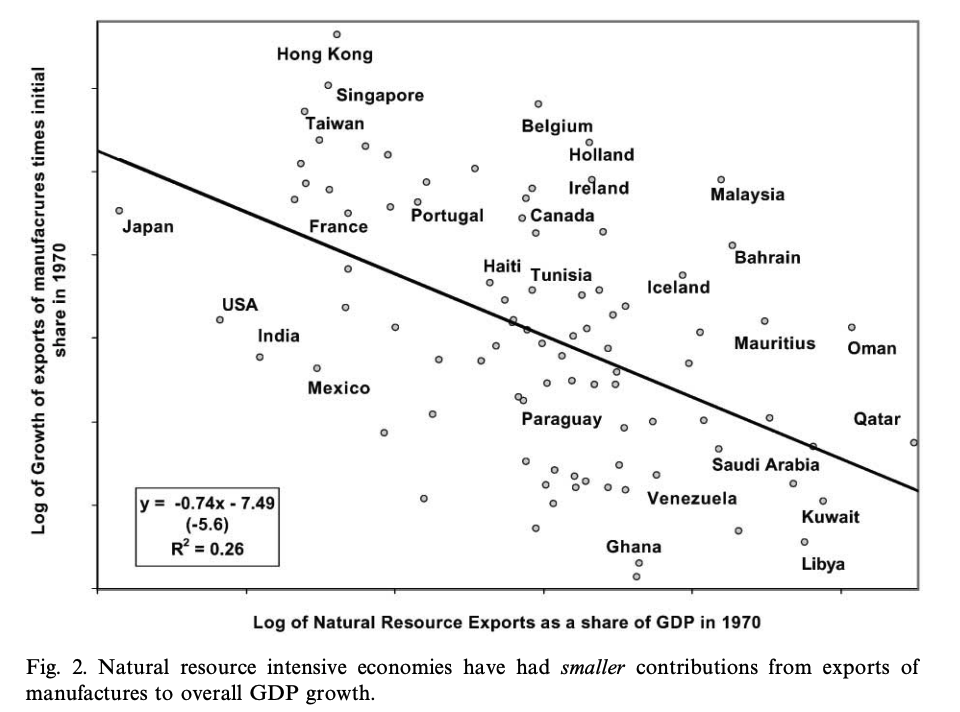
\includegraphics[width=0.5\textwidth]{../TA9/inputs/fig3.png}
\end{figure}
\begin{itemize}
\item Resource abundance tended to render the export sectors uncompetitive
\item So never successfully pursued export-led growth
\end{itemize}
\end{frame}
%---------------------------------------------------------------------

%---------------------------------------------------------------------
\begin{frame}{Possible Mechanisms III}
\begin{itemize}
\item Autocractic or oligarchic governance
\begin{itemize}
    \pause \item Elicits a political contest for resource rents
    \pause \item Extractive industries emerged 
    \pause \item Which commodities? Oil, minerals, cocoa, coffee, plantation crops
\end{itemize}
\item Anarchic institutions
\begin{itemize}
    \pause \item Unenforeceable property rights - tragedy of the commons
    \pause \item Unsustainably rapid depletion of resources - solution to privatise?
    \pause \item Civil war - factions fight for control of resources (Angola, Sudan) 
\end{itemize}
\pause \item Cyclical expansion of the non-traded sector via the Dutch Disease
\begin{itemize}
    \pause \item Currency appreciates $\rightarrow$ govt. spending $\uparrow$ $\rightarrow$ non-traded sector prices $\uparrow$ $\rightarrow$ shift of labour and land from traded to non-traded sector
    \pause \item Economy more vulnerable to resource-related shocks
\end{itemize}
\end{itemize}
\end{frame}
%---------------------------------------------------------------------

\section*{Practice Final}


\end{document}
